%%%%%%%%%%%%%%%%%%%%%%%%%%%%%%%%%%%%%%%%%%%%%%%%%%%%%%
\section{はじめに}

 地震等に伴う電離圏の変動を観測するため,HF帯電波を用いたHFD観測という手法が取られている.このHFD(短波ドップラー)観測のデータは電離圏研究のためにオープンデータとして公開されており,自由な使用が認められている.\cite{hfd_report}\\
 現状,データ活用を促進するために数件の web アプリケーションが開発されている.しかし,設計時点で複数の言語が使用されている,ページの読み込みに時間がかかるなど,その多くが開発運用の困難性やユーザーエクスペリエンス等の観点で問題を抱えている.\\
 例として,図1にHFDのオープンデータが公開されているwebサイトの一部を示す.\cite{hfd_link}\\
 \begin{figure}[h]
   \centering
   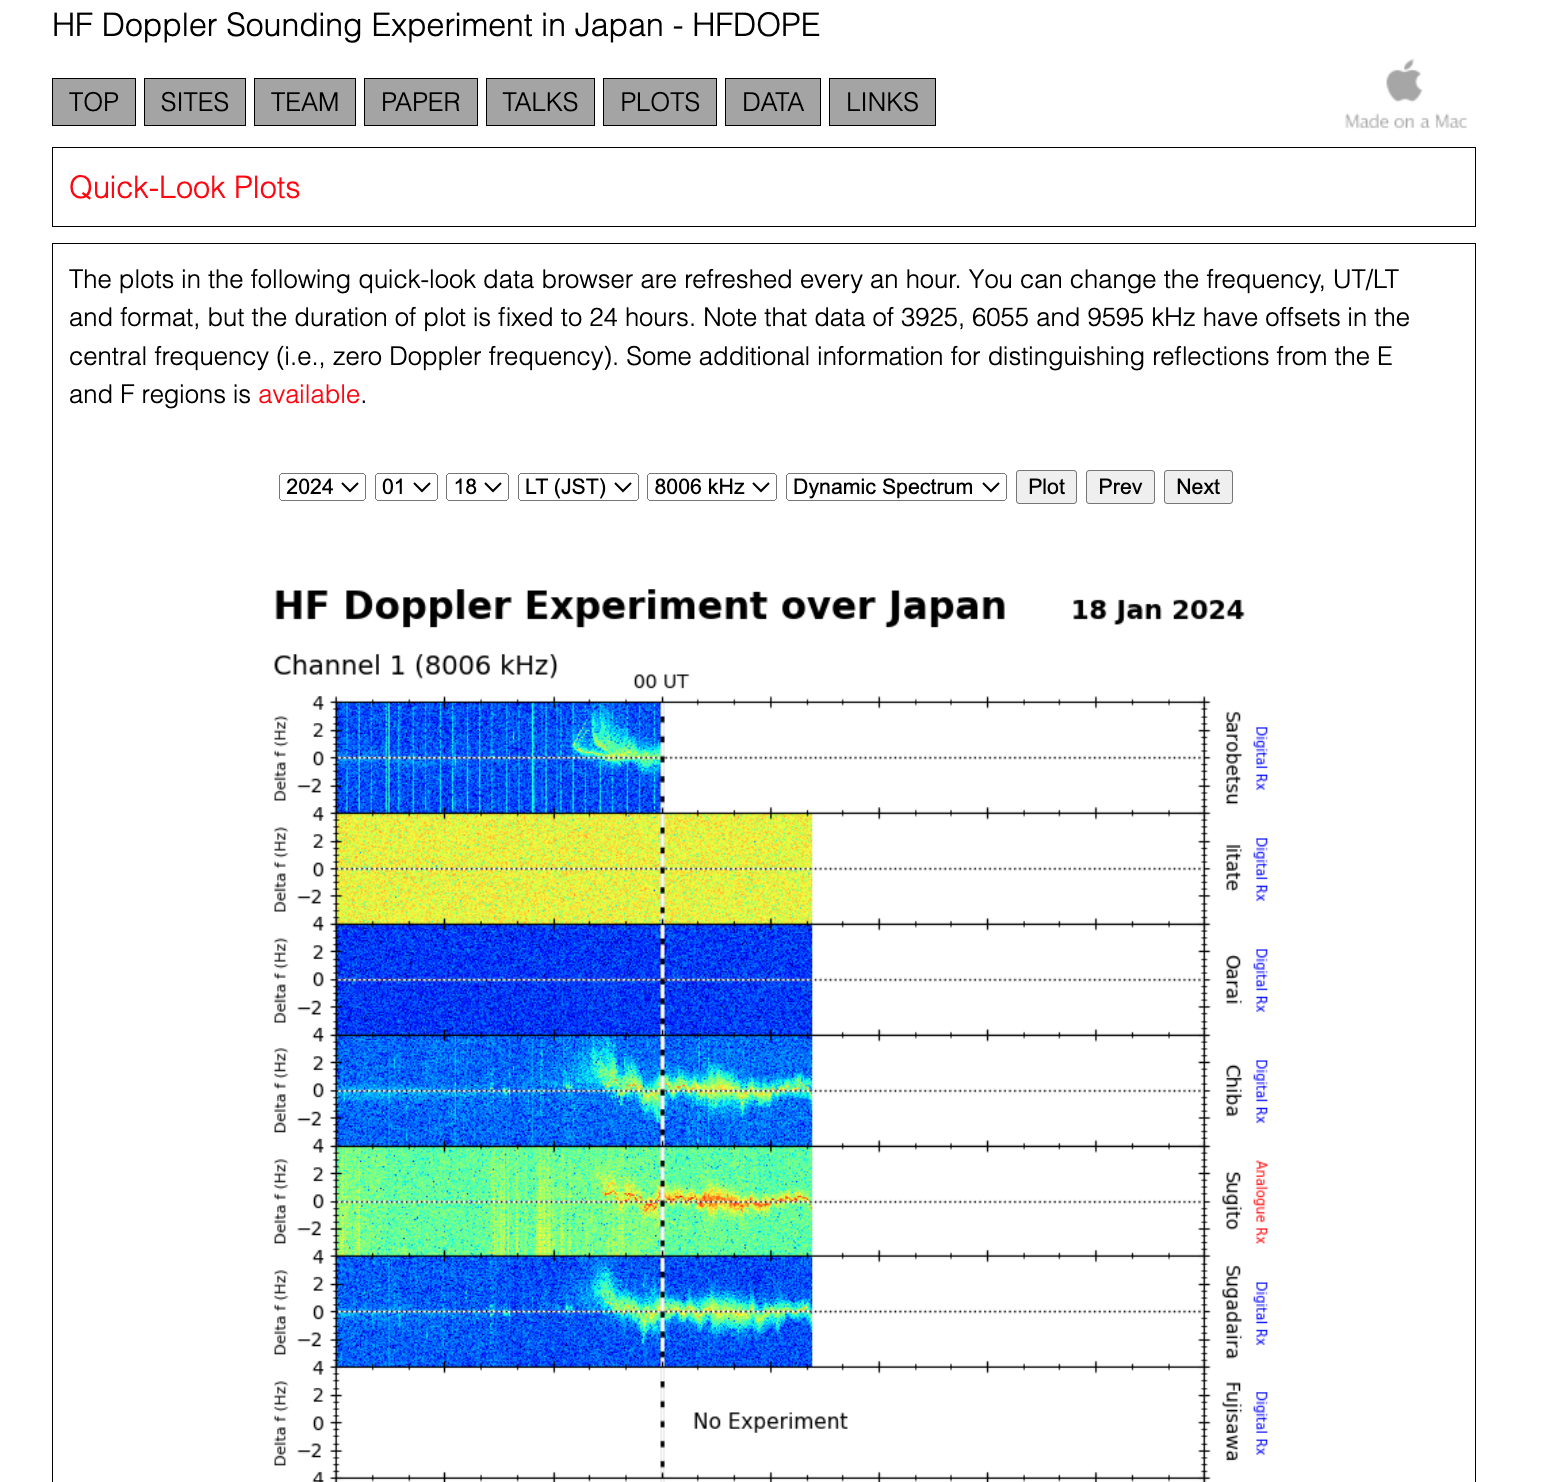
\includegraphics[width=70mm]{fig/websc.png}
   \caption{オープンデータが公開されいているwebサイト}
 \end{figure}\\
 これは,公開されているオープンデータを元にプロットされた図を表示しているページである.図に上部にあるタブから日付やチャンネルなどを変更し,プロットされるグラフのデータを変更することができる.しかし,観測年,月,,観測方法,チャンネルの周波数などを1つずつ変更する必要があるため,かなり不便になってしまっている.また,同時に1つまでしかグラフを表示することができず日付ごとの比較などが不便になってしまっている.\\
%%\textcolor{red}{ここに問題の例を具体的に記述してください}
また,webアプリケーションの主な使用者となる電離圏の研究者から,webアプリケーションの仕様についていくつかの要望が出されている.それらをいくつか抜粋して,以下表1に示す.\\
\begin{table}[h]
  \centering
  \caption{webアプリケーションに対する要望の抜粋}
  \begin{tabular}{l}
  \toprule
    ・周波数固定で全ての局を見せる\\
    ・局固定で全ての周波数を見せる\\
    ・局,周波数を選んでカスタムプロットしたい\\
    ・ダイナミックスペクトルを見たい\\
    ・PDF などの形に出力できると良い\\
    ・パンとズームができると良い
  \end{tabular}
\end{table}\\
 既存のwebアプリケーションにおける課題点の解消,及び研究者からの要望を反映したwebアプリケーションを提供するため,webアプリケーションの新規設計を行う.

\textcolor{red}{全体のシステム構成図を他のメンバーとかぶってもいいから示す}

既存のwebアプリケーションにおける課題点を解消するため,ページレンダリング手法を考慮して開発を進めていく.本研究ではNext.jsと呼ばれるJavaScriptのフレームワークを用いて実装を行う.JavaScriptのUIライブラリの一つであるReact.jsがベースとなっており,サーバ機能も有しているため効率的なweb開発が可能である.また,サーバーサイドレンダリング(SSR)や静的サイト生成(SSG)といった機能を持つwebサイトの作成を得意とする.そのため,今回開発するwebアプリケーションの要件に合致していると判断した.\cite{next}\\
 本研究ではこのwebアプリケーションにおける web スクレイピングを用いてオープンデータが公開されているwebサイトからデータを取得する処理,および,取得したデータを整形してフロントエンドで扱いやすく整形する処理に焦点を当てる.また,使用する言語をwebアプリケーション開発全体で統一して管理コストの低減を図るため,webスクレイピングに関する処理はTypeScriptを用いて行う.\\
 TypeScriptはJavaScriptに静的な型付けとクラスベースなオブジェクト指向を加えたもので,型定義を明確にできる,事前にエラーを防止できるといった利点がある.また,本開発ではアプリケーションフレームワークにNext.jsを採用する.そのため,TypeScriptが本研究でのデータ整形,出力処理に適していると判断し採用した.
%%\textcolor{red}{TypeScriptが他の言語に比べてどのような点で優れているか本研究で採用する理由をもう少し詳細にかいて説得力を持たせる}

%%%%%%%%%%%%%%%%%%%%%%%%%%%%%%%%%%%%%%%%%%%%%%%%%%%%%%
\section{Webスクレイピングについて}

 webスクレイピングとは,web サイトから情報を抽出するコンピュータソフトウェア技術のことを指す.HTML フォーマットからテキストを抽出してスプレッドシートや json ファイル等の構造化データへの変換を行うことができ,web 上にあるデータを取得して扱うことを目的とする.web スクレイピングの手法としては,正規表現や DOM 解析,HTML パーサ等を用いたものがある.本研究では,ISRを用いたwebアプリケーションを設計するため,スクレイピングの処理に速度を求める必要がない.そのため,本研究では軽量でサーバへの負担が小さいcheerioをHTMLパーサとして用いる.
%%%%%%%%%%%%%%%%%%%%%%%%%%%%%%%%%%%%%%%%%%%%%%%%%%%%%%
\section{使用ライブラリ}
 本研究で使用した主なTypeScriptライブラリについて以下に示す.
%%%%%%%%%%%%%%%%%%%%%%%%%%%%%%%%%%%%%%%%%%%%%%%%%%%%%%
\subsection{Superagent}

 HTMLリクエストを送信することのできるモジュール.非同期処理に適しており,動作が早く,負荷が軽いという利点があるため,採用した.本研究ではHFD観測データが公開されているwebページからHTMLレスポンスとしてテキストデータを取得する際に用いる.\cite{superagent}
%%%%%%%%%%%%%%%%%%%%%%%%%%%%%%%%%%%%%%%%%%%%%%%%%%%%%%
\subsection{Cheerio}

 HTMLパーサにjQueryのサブセットを実装したもの.HTMLドキュメントのタグやクラスを指定して,目的のテキストを抜き出すことができる.利点として,jQueryの関数を用いてスクレイピングの処理を行うことができる.jQueryライクに記述することがでる,動作が早く,負荷が軽い,ほぼすべてのHTMLドキュメントをパースできるという点が挙げられる.そのため,本研究では本研究ではHTMLレスポンスからテキストデータだけを抜き出す際に用いる.\cite{cheerio}
%%%%%%%%%%%%%%%%%%%%%%%%%%%%%%%%%%%%%%%%%%%%%%%%%%%%%%
\section{実装}
%%%%%%%%%%%%%%%%%%%%%%%%%%%%%%%%%%%%%%%%%%%%%%%%%%%%%%
\subsection{目標}
 本開発では,Next.jsを用いて開発運用及びユーザーエクスペリエンスの観点で従来のものよりも優れており,なおかつ主な使用者となる研究者の要望を取り入れたWebアプリケーションを新規に作成することを目標とする.本研究ではその中の,webスクレイピングを用いてオープンデータが公開されているサイトからデータを取得する処理及び,それをフロントエンドで扱いやすいように整形する処理を実装することまでを目標とする.\\
 本研究ではスクレイピングおよび,データ処理を行う関数を実装し,フロントエンドから求められているデータ様式の要件を以下表2に示す. \\
 \begin{table}[h]
  \centering
  \caption{データ様式の要件}
  \begin{tabular}{l}
  \toprule
     ・json形式にまとめられている\\
     ・"hour","minute","second"という3つの\\
      プロパティを含んでいる"time"プロパティを持つ\\
     ・チャンネルの周波数ごとに"freq"と"amp"が\\
      まとめられたプロパティ,"channel"を持つ\\
  \end{tabular}
\end{table}
%%\textcolor{red}{フロントから求められているデータ様式の要件をどこかで書いておいた方がいい}
%%%%%%%%%%%%%%%%%%%%%%%%%%%%%%%%%%%%%%%%%%%%%%%%%%%%%%
\subsection{スクレイピング処理}
\textcolor{red}{どうやって発火するのか書く}
 SuperagentのGET関数を用いて,HFドップラーのデータが公開されているwebサイト\cite{hfd_link}にHTMLリクエストを送り,webサイトのHTMLリソースを取得する.例として,2020/11/20Sarobetsuのデータを示す.図1はSuperagentを用いて取得したwebサイトのHTMLリソースの一部である.\\
\begin{figure}[h]
  \centering
  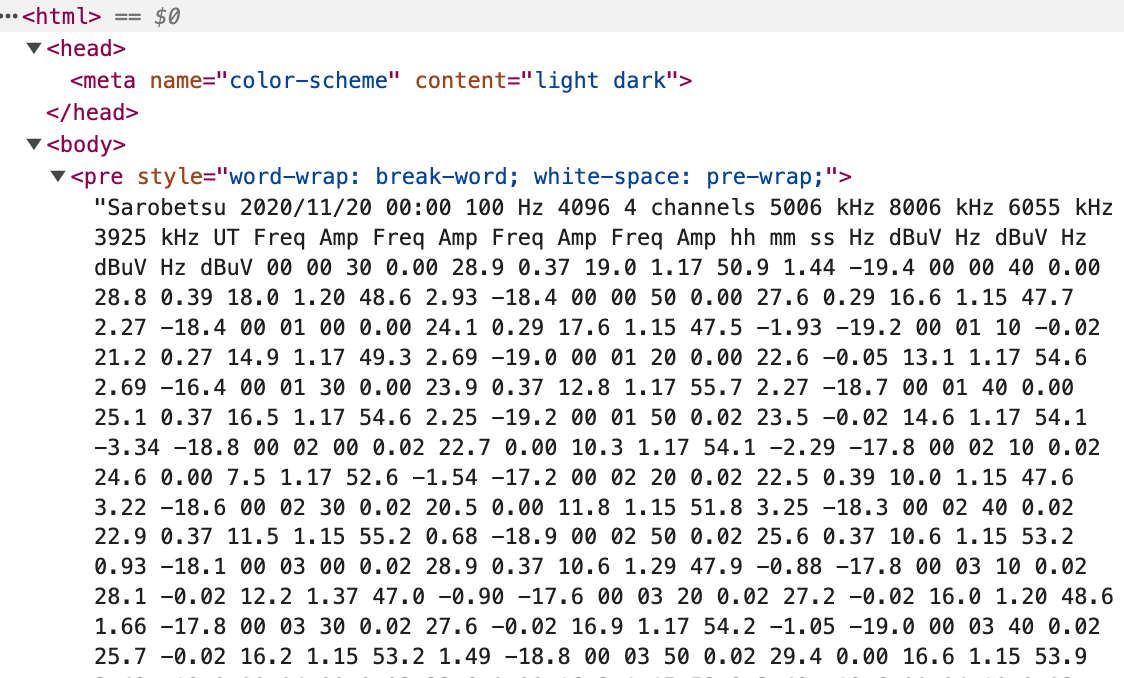
\includegraphics[width=80mm]{fig/htmlRes.png}
  \caption{サイトのHTMLリソース}
\end{figure}\\
このHTMLリソースから,cheerioを用いて目的のテキストデータのみを取り出す.今回はbodyすべてを取り出して,そのテキストデータをフロントエンドから求められているデータ様式の要件に沿って整形していく.\\
図2にHTMLリソースから取り出したデータの一部を示す.
\begin{figure}[h]
   \centering
   \includegraphics[width=70mm]{fig/textData.png}
   \caption{抜き出したテキストデータ}
\end{figure}
%%%%%%%%%%%%%%%%%%%%%%%%%%%%%%%%%%%%%%%%%%%%%%%%%%%%%%

\subsection{データ整形処理}
 \subsubsection{テキストデータを改行ごとに区切る}
 TypeScriptのsplit関数を用いてテキストデータを改行ごとに区切り,splitLineDataという配列に格納する.split関数はテキストに対して使用することができ,引数に渡した文字ごとにテキストを区切って配列にすることができる.今回は"\textbackslash n"を引数に渡すことで,改行ごとにテキストデータを区切り配列に格納する.\\
 図3にsplitLineDataの一部を示す.\\
 \begin{figure}[h]
   \centering
   \label{fig:my_label}
   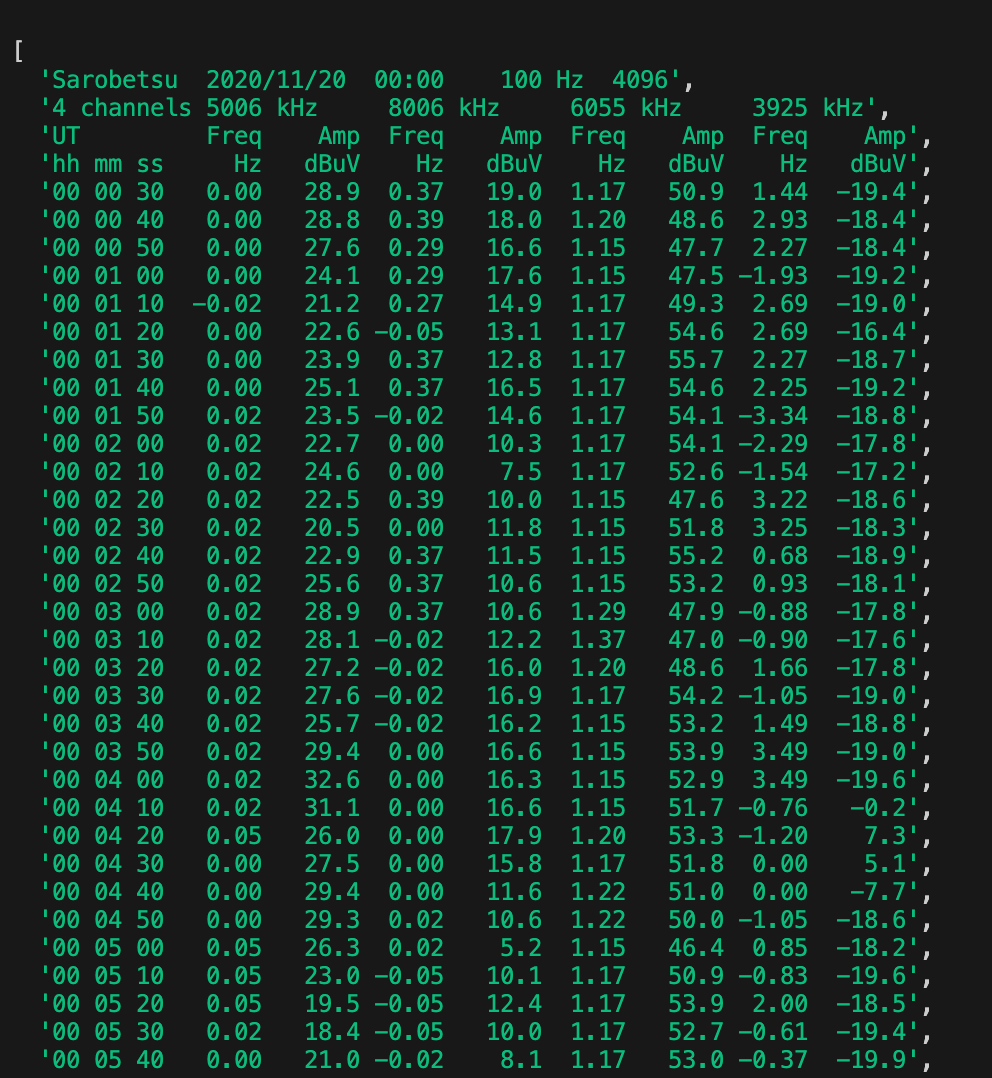
\includegraphics[width=70mm]{fig/splitLineData.png}
    \caption{改行ごとに区切ったデータ}
 \end{figure}
 %%%%%%%%%%%%%%%%%%%%%%%%%%%%%%%%%%%%%%%%%%%%%%%%%%%%%%
 
 \subsubsection{データのラベルを取り出し,テキストデータのうちラベルにあたる最初の4行を削除する}
 TypeScriptのslice関数を用いて,ラベルが記述されているsplitLineDataの2行目を取り出してlabelItemという配列に格納する.slice関数は元の配列に影響を及ぼさないため,このような場合には適している.\cite{mdn_slice}このデータは観測地点によってチャンネル数が異なっているため,チャンネル数に応じて処理を変える必要がある.それぞれテキストデータの2行1文字目にチャンネル数が記述されているため,labelItemの0番目の要素を数値に変換してnumber型の定数Nに格納する.
 ラベルから必要なデータを抜き出したため,必要の無くなったテキストデータのラベル4行をsplice関数を用いて削除し,spliceData関数に格納する.\\
 図4にspliceDataの一部を示す.\\
 \begin{figure}[h]
   \centering
   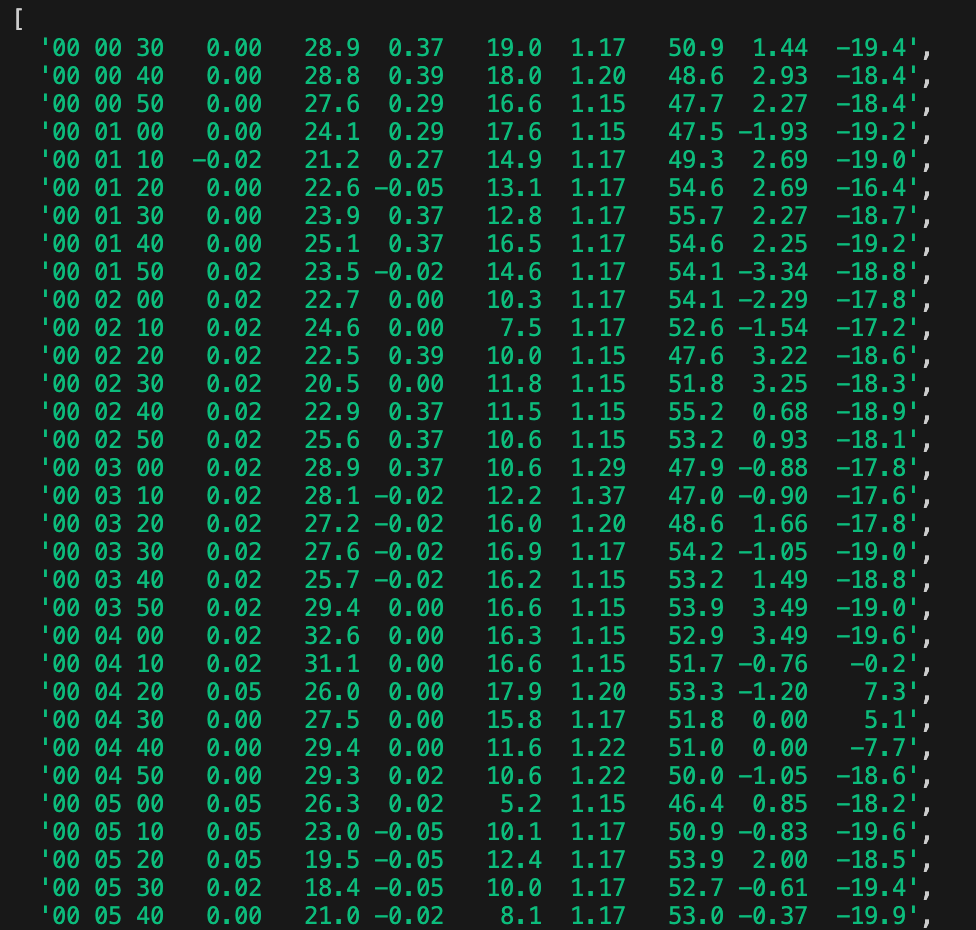
\includegraphics[width=70mm]{fig/spliceData.png}
   \caption{ラベル部分を削除したデータ}
 \end{figure}
 %%%%%%%%%%%%%%%%%%%%%%%%%%%%%%%%%%%%%%%%%%%%%%%%%%%%%%
 
 \subsubsection{データを空白ごとに区切り,配列に格納する}
 TypeScriptのmap関数を用いて,spliceDataの要素ひとつひとつに対してそれぞれsplit関数で処理を行う.splitData関数の要素,つまり改行で区切ったテキストデータは空白で区切って記述されている.そのため,split関数を用いて空白ごとに区切り,二重配列splitSpaceDataに格納する.このデータは空白1つで区切られている場合と空白2つ場合があり,そのまま格納してしまうと空白の要素が生まれてしまう.そのため,filter関数を用いて空白のみの要素を取り除く.filter関数は配列に格納する際に用い,指定された要件に合った要素以外を排除することができる.今回は,filter関数に空白(" ")を渡し,さらに要素の長さが1に満たない要素を排除することで,空白のみの要素を取り除いている.
 図5にsplitSpaceDataの一部を示す.
 \begin{figure}[h]
   \centering
   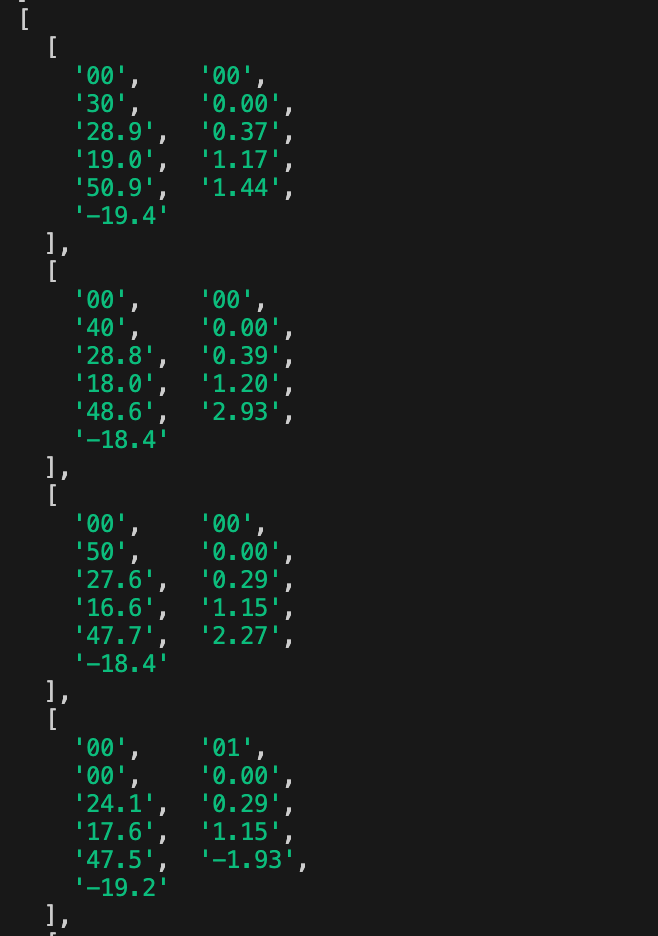
\includegraphics[width=70mm]{fig/splitSpaceData.png}
   \caption{空白ごとに区切ったデータ}
 \end{figure}
 %%%%%%%%%%%%%%%%%%%%%%%%%%%%%%%%%%%%%%%%%%%%%%%%%%%%%%
 
 \subsubsection{データを数値に変換する}
 splitSpaceData配列に格納されている要素全てを,string型からnumber型に変換する.splitSpaceData配列は二重配列であるため,二重にmap関数をかけることで要素全てをnumber型に変換し,NumberData配列に格納する.
 %%%%%%%%%%%%%%%%%%%%%%%%%%%%%%%%%%%%%%%%%%%%%%%%%%%%%%
 
 \subsubsection{データをjsonファイルに出力}
 NumberDataを,フロントエンドから求められているデータ様式の要件に沿うようにjsonファイルに出力する.今回は,Number配列をforEach関数を用いて処理する.forEach関数はmap関数と同じコールバック関数で,jsonを扱うこともできる.forEach関数は内部にvalueとindexという変数を持つことができ,valueが配列やjsonの要素のうち今扱っているものを,indexが今扱っている要素が配列やjsonのうち何番目かをそれぞれ表している.今回の場合,valueはNumber配列の中の配列になるため,テキストデータの改行1つ分を空白で区切った配列となる.
 Number配列は,二重配列の中の要素が,0番目の要素から順に"hour","minute","second","freq","amp","freq","amp"...となる配列になっている.観測地点ごとにチャンネルの数および周波数が異なるため,"freq"と"amp"の組み合わせがいくつあるかはデータによって異なる.そのため,value[0]〜value[2]をそれぞれjsonファイルのtimeプロパティの"hour","minute","second"に格納する.value[3]からは,"freq"と"amp"の2つごとにlabelItemの偶数番目に格納されているチャンネルの情報をもとにjsonに格納する.\\
 全ての要素に対して上記の処理を行ったのち,jsonをファイルに出力する.\\
生成したjsonの一部を図6に示す.\\
\begin{figure}[h]
  \centering
  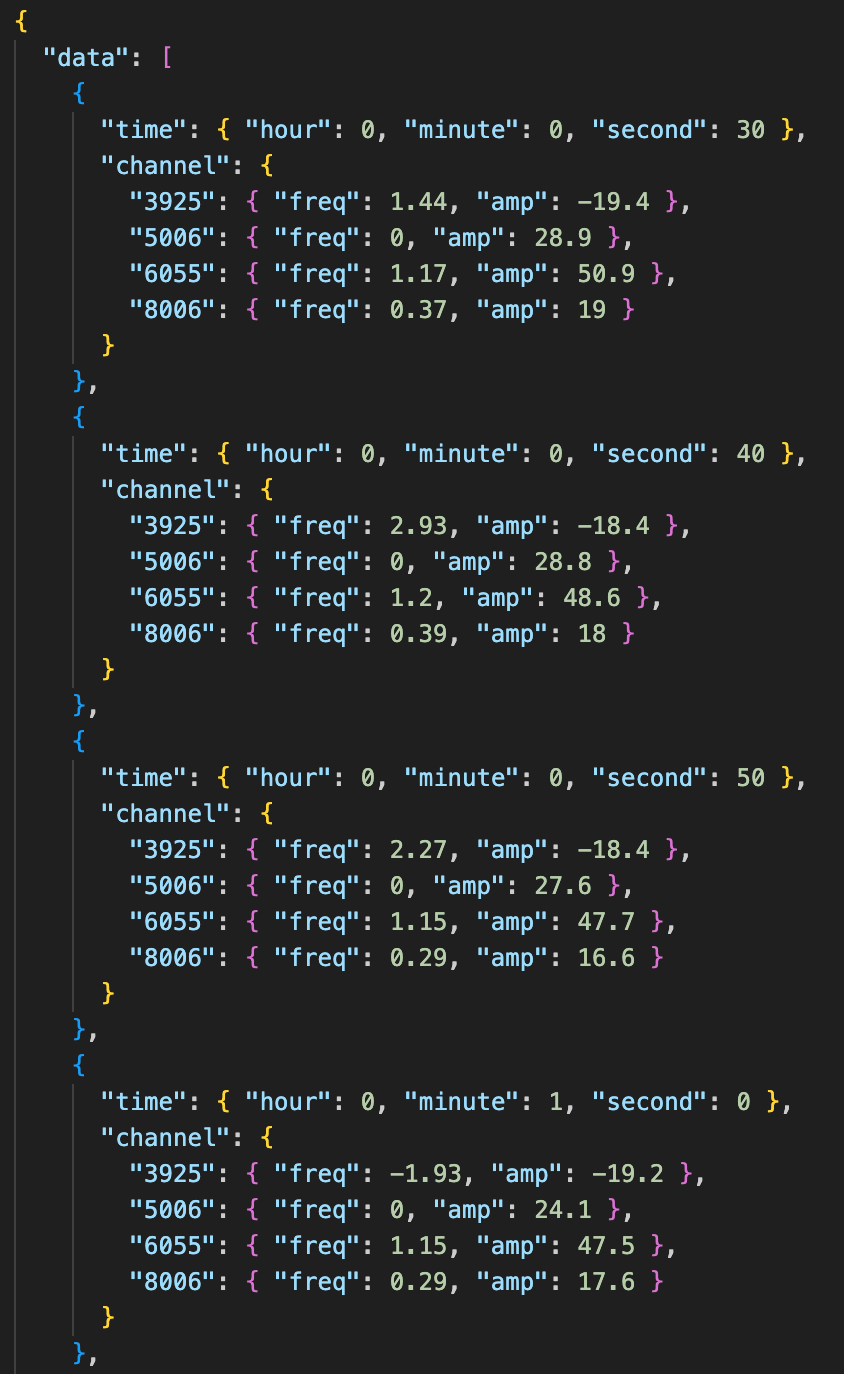
\includegraphics[width=70mm]{fig/jsonData.png}
  \caption{生成したjson}
\end{figure}
 %%%%%%%%%%%%%%%%%%%%%%%%%%%%%%%%%%%%%%%%%%%%%%%%%%%%%%

 %%\textcolor{red}{ここら辺が藤本君が研究で工夫した点になると思うので、技術的な壁があったのか、あったならどうやって対応したのか、壁がなかったらこの研究の新規性が整形処理のどのあたりにあるのか書く}

%%%%%%%%%%%%%%%%%%%%%%%%%%%%%%%%%%%%%%%%%%%%%%%%%%%%%%
\subsection{今回のデータ整形処理について}
 このオープンデータは観測地点によってチャンネルの数および周波数が異なり,それに応じて処理の内容と出力するjsonファイルのプロパティ名を変更する必要がある.\\
 データ整形処理の実装当初,この観測地点ごとのチャンネルの違いについてあらかじめjsonの型定義に全ての周波数分のプロパティを用意しておき,必要に応じて利用するという方法を試みた.しかし,その方法では出力したデータファイルに無駄が多く,データファイルを閲覧する際の視認性が悪く,データファイルを保存する際に容量を圧迫してしまうため好ましくない.\\
 そのため,元データのラベル部分をあらかじめデータ整形用の配列とは別に保存しておき,json生成の際に利用することで観測地点ごとにチャンネルの数と周波数ごとに適切な処理を行う方法をとった.\\
 また,当初はjsonの構成でデータ部分を"channel"プロパティにまとめずそのまま周波数ごとに記述していた.しかし,観測地点ごとにチャンネルの数および周波数が違う今回の場合ではその方法ではフロントエンドで扱いづらく,また可読性等の観点で好ましいデータ様式ではないため上記表2にように"time"プロパティと"channel"プロパティを分けることとした.
\subsection{完成品}
 完成したサイトがこちらになります.
%%\textcolor{red}{たくさん図を貼った方がいいですね}
%%%%%%%%%%%%%%%%%%%%%%%%%%%%%%%%%%%%%%%%%%%%%%%%%%%%%%
\small
\begin{thebibliography}{99}
\setlength{\itemsep}{0pt}
\smallskip

\bibitem{hfd_report}
吉川晃平,HFドップラーにより観測された地震に伴う電離圏変動の中性待機波導数値シミュレーションによる定量的評価,電気学会論文誌A Vol.136 No.5 pp.259~264

\bibitem{next}
Next.js by Vercel - The React Framework
\url{https://nextjs.org/} 2024/1/13

\bibitem{shu_sotsuken}
中嶋柊,HF ドップラー観測データの利活用を目的とする web アプリケーションのフロントエンド設計,令和4年度 制御情報システム創造演習 報告書

\bibitem{superagent}
Superagent-npm 
\url{https://www.npmjs.com/package/superagent}  2023/01/25

\bibitem{cheerio}
cheeriojs/cheerio: Fast, flexible, and lean implemenhttps://developer.mozilla.org/ja/docs/Web/JavaScript/
Reference/GlobalObjects/Array/mapt ation of core jQuery designed specifically for the server. 
\url{https://github.com/cheeriojs/cheerio}  2023/01/25 

\bibitem{hfd_link}
HF Doppler Sounding Experiment in Japan - HFDOPE
\url{http://gwave.cei.uec.ac.jp/~hfd/pre.html} 2024/1/13

\bibitem{mdn_splice}
Array.prototype.splice() - JavaScript | MDN
\url{https://developer.mozilla.org/ja/docs/Web/JavaScript/Reference/Global_Objects/Array/splice} 2024/1/13

\bibitem{mdn_slice}
Array.prototype.slice() - JavaScript | MDN
\url{https://developer.mozilla.org/ja/docs/Web/JavaScript/Reference/Global_Objects/Array/slice} 2024/1/13

\bibitem{mdn_map}
Array.prototype.map() - JavaScript | MDN
\url{https://developer.mozilla.org/ja/docs/Web/JavaScript/Reference/Global_Objects/Array/map}
2024/1/13

\bibitem{mdn_filter}
Array.prototype.filter() - JavaScript | MDN
\url{https://developer.mozilla.org/ja/docs/Web/JavaScript/Reference/Global_Objects/Array/filter} 2024/1/13

\bibitem{mdn_horEach}
Array.prototype.forEach() - JavaScript | MDN
\url{https://developer.mozilla.org/ja/docs/Web/JavaScript/Reference/Global_Objects/Array/forEach} 2024/1/13

\end{thebibliography}
\normalsize
%%%%%%%%%%%%%%%%%%%%%%%%%%%%%%%%%%%%%%%%%%%%%%%%%%%%%%